%%%% MACRO DEFINITION %%%%

\providecommand{\pvivax}{P.~vivax}
\providecommand{\pfalciparum}{P.~falciparum}
\providecommand{\cterm}{C-terminus}
\providecommand{\nterm}{N-terminus}

\providecommand{\e}[1]{\ensuremath{\times 10^{#1}}}
\newcolumntype{P}[1]{>{\centering\arraybackslash}p{#1}}
\newcolumntype{M}[1]{>{\centering\arraybackslash}m{#1}}

\providecommand{\refimage}[1]{\figurename~\ref{fig:#1}}

%TC:macro \note [ignore]



%%%%%%%%%%%%%%%%%%%%%%%%%%%%%%%%%%%%%%%%%%%%%%%%%%%%%%%%%%%%%%%%%%%%%%%%%%%%%%%%%%%%%%%%%%%%%%%%%%%%%%%%%%%%%%%%%%%%%
%%%%%%%%%%%%%%%%%%%%%%%%%%%%%%%%%%%%%%%%%%%%%%%%%%%%%%%%%%%%%%%%%%%%%%%%%%%%%%%%%%%%%%%%%%%%%%%%%%%%%%%%%%%%%%%%%%%%%
%													BEGIN
%%%%%%%%%%%%%%%%%%%%%%%%%%%%%%%%%%%%%%%%%%%%%%%%%%%%%%%%%%%%%%%%%%%%%%%%%%%%%%%%%%%%%%%%%%%%%%%%%%%%%%%%%%%%%%%%%%%%%
%%%%%%%%%%%%%%%%%%%%%%%%%%%%%%%%%%%%%%%%%%%%%%%%%%%%%%%%%%%%%%%%%%%%%%%%%%%%%%%%%%%%%%%%%%%%%%%%%%%%%%%%%%%%%%%%%%%%%

\chapter{Predicting Zinc Binding Sites} % Write in your own chapter title
\label{Chapter4}
\lhead{Chapter 4. \emph{Predicting Zinc Binding in Proteins}} % Write in your own chapter title to set the page header

The aim of this part of the PhD is to create a system which conceptually is quite simple --- it would take as its input a protein sequence or protein sequence, and output a list of zero or more residue combinations which are predicted to form a zinc binding site, with an accompanying probability.

This system is a machine learning system - it uses binary classifiers trained on the large dataset of zinc binding sites described in the previous chapter which `learn' what zinc binding sites look like from that data.

This chapter will describe the approach taken to solving this problem, the models created, the architecture of the system from the user's point of view, and how the models are accessed and used.

\section{Approach}

As explored in Chapter 2, there have been multiple studies in the past which have used machine learning (or simpler methods) to create zinc-binding predictors (or general-purpose metal-binding predictors). Many of the general principles of these studies are adopted here, however there are two crucial methodological changes that I have chosen to make.

One recurring feature of these previous works, particularly in the sequence-based predictive models, is the focus on zinc binding \emph{residues} rather than zinc binding \emph{sites}. In most cases, the entity examined by the predictive model is the individual residue, often with a surrounding linear sequence `window' of residues. The model then assigns a probability as to whether that residue is a zinc binding residue. As outlined in that chapter, this approach has had a measure of success, but it is a somewhat artificial concept. There is, after all, no such thing as a zinc-binding residue in isolation. The individual residues of a high-affinity zinc binding site of the kind considered here are only zinc-binding when the other residues are present, and conversely many non-zinc-binding residues could bind zinc if other residues were present in the correct locations. It is particular \emph{combinations} of residues, not individual residues, which are zinc binding --- an important fact not usually considered in research of this kind. As this chapter will explain, I have opted to create models which inspect residue combinations, not single residues.

Another commonality is the treatment of zinc binding sites as a single category, and the presumption of properties that are common to them all regardless of the residues of which they are comprised. This may well be sufficient --- particularly as there are essentially only four residues that make up the vast majority of zinc binding sites --- but it is possible that properties used for prediction have much tighter distributions within particular sub-categories of zinc binding sites. As such, I have elected not to create a single model that predicts zinc binding in structures and another that predicts them in sequence, but rather one model per \emph{family} of zinc binding site, of the kind described in Chapter 3. That is, there is a model for predicting H3 binding sites (those made of three histidine residues) in structure, one for predicting H3 binding sites in sequence, one for predicting C2H2 binding sites in structure, for predicting C2H2 sites in sequence, and so on. As well as the increased specificity this affords, another advnatage of this approach is a purely practical one. All the possible H3 binding sites in a protein are found by taking all combinations of three histidine residues, and while the combinatorics of this can lead to large numbers of potential sites to check, it is vastly smaller than the combinations of \emph{all} residues that would need to be checked if the model was suppoed to look for a generic zinc binding sites --- an infeasible task for all but the smallest of proteins.

The overall pipeline of the resulting system for predicting zinc binding then, is that when a protein structure of sequence is given, for each family for which there is a model all residue combinations within that protein which match the family are identified (all unique combinations of three histidine residues for H3, for example) and passed to the relevant model, which assigns a probability that the residues comprise a zinc binding site, as well as making a binary yes-or-no prediction. This is repeated for every combination, and for every family, to build up a list of predicted binding sites.

\section{Data Preparation}

The first decision to make was which families to use. There are 701 families in total in ZincBind, ranging from C4 with its 3069 unique representatives, to obscure families like C1D1E1H2 (one cysteine, one glutamate, one aspartate and two histidine residues) which has only one representative. In fact there are 244 families with one representative, and many with only a small number of representatives. To train a model that can recognise some combination of residues as being a zinc binding site of some family rather than some random combination, the model needs to be trained on many, many examples of such sites so there is clearly a minimum number of representatives in the database that a family must have for it to make sense to train a model for it. It is not immediately obvious what this minimum number should be. Initially I decided to use the top ten families --- C4, C3H1, C2H2, D1H2, E1H2, H3, C3, E1H1, C2H1 and D1H1. This was originally a somewhat arbitrary cutoff and the intention was to adjust it based on results, though as this chapter will show, ten families is probably the correct number in terms of resultant dataset size.

For a binary classifier of the kind being created here, the training set is a collection of positive samples (combinations of residues of that family which represent zinc binding sites) and negative samples (combinations of residues of that family which are not zinc binding sites). An assumption being made here is that if a combination of residues does not have a zinc atom bound to it in a structure, it is not a zinc binding site. This may not be true occasionally, as the structure simply may not have been crystallised in the presence of zinc. For this reason, some of the negative samples in the training sets may actually be positive. It is assumed however, that these cases are sufficiently infrequent as to have a negligible effect.

The residue combinations are represented in the training data as a vector of measurements, with the final measurement being the indicator of whether it is positive (1) or negative (0). Each row in the training data represents a residue combination, each column a feature. There are twenty training datasets altogether --- for each of the ten families there is a training set for sequence data and a training set for structural data.

\subsection{Sequence Training Data}

To generate the sequence training datasets, for each family the ZincBind API was queried for all binding sites of that family, and those split over multiple chains were removed to leave single sequence binding sites --- the multi-chain zinc binding sites do not have a single sequence containing all the necessary residues in the combination. The resulting sequences were turned into feature vectors which contained the number of residues between each pair of binding residues, the average hydrophobicity of residues either side of the binding residues, using windows of size 1, 3 and 7, and the average number of charged residues either side of the binding residues, using the same window sizes. This created a dataset of positive samples.

For the negative samples, for each family a sequence was chosen at random from the set of all unique sequences in UniProtKB and a combination of residues within that sequence matching the family but not a known binding site, was selected --- this was done repeatedly until a list of negative samples was built up equal in size to the
positive dataset.  The two datasets were combined into a single dataset for each family. The resultant dataset is summarised in Table~\ref{tab:dataset-size}.

\subsection{Structure Training Data}

To generate the structure training datasets, for each zinc-binding family, all relevant zinc binding sites belonging to a PDB structure with resolution better than 2~{\AA}ngstr\"{o}ms were downloaded --- as many of the measurements made are geometric, precise atom distances are important, and structures with too poor a resolution would create unreliable data for this purpose. For each PDB entry, the structure was downloaded and parsed using the Python library atomium (see Appendix A), assembled into the correct biological assembly, and then each binding site was turned into a feature vector using the following measurements: mean inter C$\alpha$ distance of the liganding residues, standard deviation of the C$\alpha$ distances, minimum C$\alpha$ distance, maximum C$\alpha$ distance --- and the corresponding measurements for the C$\beta$ atoms, for a total of 8 geometric features. The distances used are all the pairwise combinations of the atoms involved, so H3 sites will have three inter C$\alpha$ distances, C4 sites will have six, and so on. The final feature is the `hydrophobicity contrast function', calculated at the centre of the C$\beta$ atoms with a radius of 7~{\AA}ngstr\"{o}ms, This algorithm is a measure of how much outer atoms in a sphere are more hydrophobic than inner atoms, with higher values previously shown to be associated
with centres of metal binding \cite{yamashita1990metal,gregory1993prediction}, as covered in Chapter 1.

As with the sequence data, this was repeated on combinations of residues with no known zinc binding ability until there was an equal number of negative samples. For these, PDB structures with no zinc atoms were selected at random (random sampling with replacement), and any random matching combination of residues from within was selected. The resultant dataset is summarised in Table~\ref{tab:dataset-size}.

\begin{table}
  \caption{\label{tab:dataset-size}The sizes of the twenty training set sizes used to train the models. In each case the size is less than the theoretical maximum of double the total number of sites per family, because the sequence sites have those with multiple chains filtered out, and the structure sites have those from poor resolution structures filtered out.}
\begin{center}
\begin{tabular}{lll} \hline
Family & Structure Dataset Size & Sequence Dataset Size \\ \hline
C4     & 2825         &  15332  \\
C3H1   & 3232         &  9158   \\
H3     & 3078         &  4524   \\
E1H2   & 1287         &  2574   \\
C2H2   &  702         &  3715   \\
D1H2   &  982         &  2406   \\
C3     &  407         &  2591   \\
C2H1   &  506         &  1926   \\
D1H1   &  522         &  804    \\ 
E1H1   &  416         &  812    \\ \hline
\end{tabular}
\end{center}
\end{table}

\section{Model Training}

While the quality and size of the training set is a large determinate of eventual model quality, the choice of machine learning algorithm is also crucial. Chapter 2 explored the history of metal binding site predictive models and the various algorithms used --- as expanded upon there, there has been a shift towards the use of deep learning models over the past five years, partly driven by the widespread adoption of backpropagation which made it practical to train large neural networks. However another reason behind this shift has been the vast increase in the size of available datasets, which are generally required for something which uses as many layers of abstraction as neural networks. As the datasets here are necessarily quite small compared with those datasets (a deliberate tradeoff made in the hopes of creating highly specific models), I decided that such algorithms were not appropriate.

I therefore considered K-Nearest Neighbor, Support Vector Machines, and Random Forest algorithms. Originally, the intention was to train a model with each of these algorithms and have the final model be a consensus of these three whereby they vote on each incoming residue combination. However early testing showed that Random Forest so consistently and significantly outperformed both the other two models in isolation, and the resultant consensus model, that I ultimately decided to solely use Random Forest for training.

The actual training of the models was done using the Python library scikit-learn \cite{scikit-learn}. For each training dataset, the data was randomly split into training and test data using an 80:20 split --- the former used to train, the latter used to evaluate. As explained in chapter 2 this is vital to ensure the resultant model is not overfit.

The hyper-parameters for each model were selected separately using 5-fold cross validation of the training set. The hyper-parameters explored were the impurity measure (gini \emph{vs.} entropy --- the algorithm used to split individual trees at each node), the maximum depth that the component trees could have (4, 6, 8 or no maximum), the number of trees in the forest (10, 100 or 1000), and the means of determining the best number of features at each split (either the
square root of the number of features, or the log$_2$ of the number of features). Once optimal hyper-parameters were identified (determined by which combination produced the best MCC score in the cross-validation), the models were trained with those hyper-parameters using the entire training dataset.

Once the model was trained on the ideal hyperparameters using all the training data, the model was evaluated on the test data, and the true positive, false positive, true negative and false negative counts were calculated. From these the recall, precision, F1 score, and Matthew's Correlation Coefficient were calculated. All of these were saved to the model by making them properties of the actual Python object, and then this Python object was serialised to disk using the Python `joblib' library for later use.

\section{Model Performance}

For the structural models, the lowest MCC score was 0.88 (for the E1H1 model). This, and the D1H1 model (MCC=0.91), relies on the geometry between just two residues, which makes creating a distinct separation between the two classes somewhat more difficult --- though their performance is still very close behind the three and four residue family models. The structure models had an average MCC of 0.960 (see Table~\ref{tab:structure}).

The sequence models also had high scores, though were more variable. The four residue sites in particular had highly conserved patterns of residue spacing and flanking hydrophobicity despite being from several homologous families. The average MCC score for the sequence models was 0.87, with the lowest MCC being 0.61 for the E1H1 model and 0.74 for the D1H1 model --- again the two two-residue models were some way behind the MCC of 0.84 for the C3 model (see Table~\ref{tab:sequence}).

The high performance of the models appears to justify the methodological changes made compared with previous metal binding classifiers. The performance scores here compare favorably with recent comparable predictive models based on structure and sequence covered in Chapter 2 --- most notably the `SVM and Sample-weighted Probabilistic Neural Network' (MCC$=0.80$) \cite{li2019}, the `meta-zinc predictor' (MCC$=0.79$) \cite{li2017} and ZincExplorer (MCC$=0.78$) \cite{chen2013}.

\begin{table}
  \caption{\label{tab:structure}Results for structure models, sorted
    by Matthews Correlation Coefficient (MCC). The two-residue
    families' performance was lower than the others as there is
    essentially just the measurements between two centres to perform
    the classification, but still scored relatively
    highly. Four-residue sites in particular were found to have very
    predictable properties.}
\begin{center}
\begin{tabular}{llllll} \hline
Family & Dataset Size & Recall & Precision & F1    & MCC  \\ \hline
C2H2   &  702         & 1.00   & 1.00      & 1.00  & 1.00 \\
C4     & 2825         & 1.00   & 1.00      & 1.00  & 1.00 \\
C3H1   & 3232         & 1.00   & 0.99      & 1.00  & 0.99 \\
E1H2   & 1287         & 1.00   & 0.99      & 1.00  & 0.99 \\
C2H1   &  506         & 1.00   & 0.98      & 0.99  & 0.98 \\
H3     & 3078         & 1.00   & 0.98      & 0.99  & 0.98 \\
D1H2   &  982         & 1.00   & 0.98      & 0.99  & 0.98 \\
C3     &  407         & 1.00   & 0.98      & 0.99  & 0.98 \\
D1H1   &  522         & 1.00   & 0.91      & 0.95  & 0.91 \\ 
E1H1   &  416         & 0.93   & 0.95      & 0.94  & 0.88 \\ \hline
\end{tabular}
\end{center}
\end{table}

\begin{table}
\caption{\label{tab:sequence}Results for sequence models, sorted by
  Matthews Correlation Coefficient (MCC).}
\begin{center}
\begin{tabular}{llllll} \hline
Family & Dataset Size & Recall & Precision & F1    & MCC  \\ \hline
C4     & 15332        & 1.00   & 0.98      & 0.99  & 0.98 \\
H3     & 4524         & 0.98   & 0.99      & 0.98  & 0.97 \\
C2H2   & 3715         & 0.97   & 0.99      & 0.98  & 0.95 \\
C3H1   & 9158         & 0.98   & 0.96      & 0.97  & 0.94 \\
E1H2   & 2574         & 0.95   & 0.97      & 0.96  & 0.92 \\
D1H2   & 2406         & 0.94   & 0.95      & 0.94  & 0.90 \\
C2H1   & 1926         & 0.93   & 0.95      & 0.94  & 0.88 \\
C3     & 2591         & 0.95   & 0.89      & 0.92  & 0.84 \\
D1H1   & 804          & 0.80   & 0.93      & 0.86  & 0.74 \\
E1H1   & 812          & 0.81   & 0.83      & 0.82  & 0.61 \\ \hline
\end{tabular}
\end{center}
\end{table}

\begin{figure}
\centering
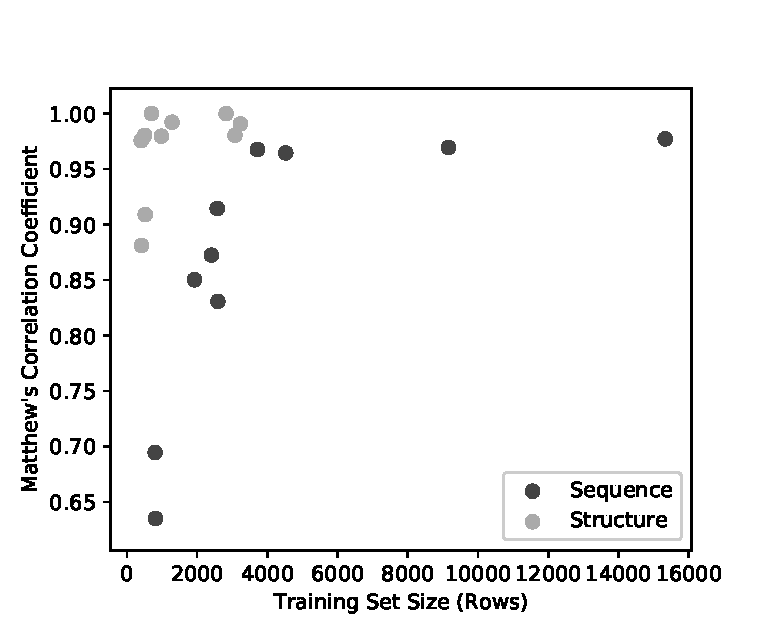
\includegraphics[width=1.0\textwidth]{Figures/size-score.eps}
\caption{\label{fig:size-score} Model Performance (MCC) as a function
  of training set size. Below ~4,000 rows, performance declines
  sharply, though above this threshold there ceases to be a strong
  correlation between the two.}
\end{figure}


\begin{figure}
\centering
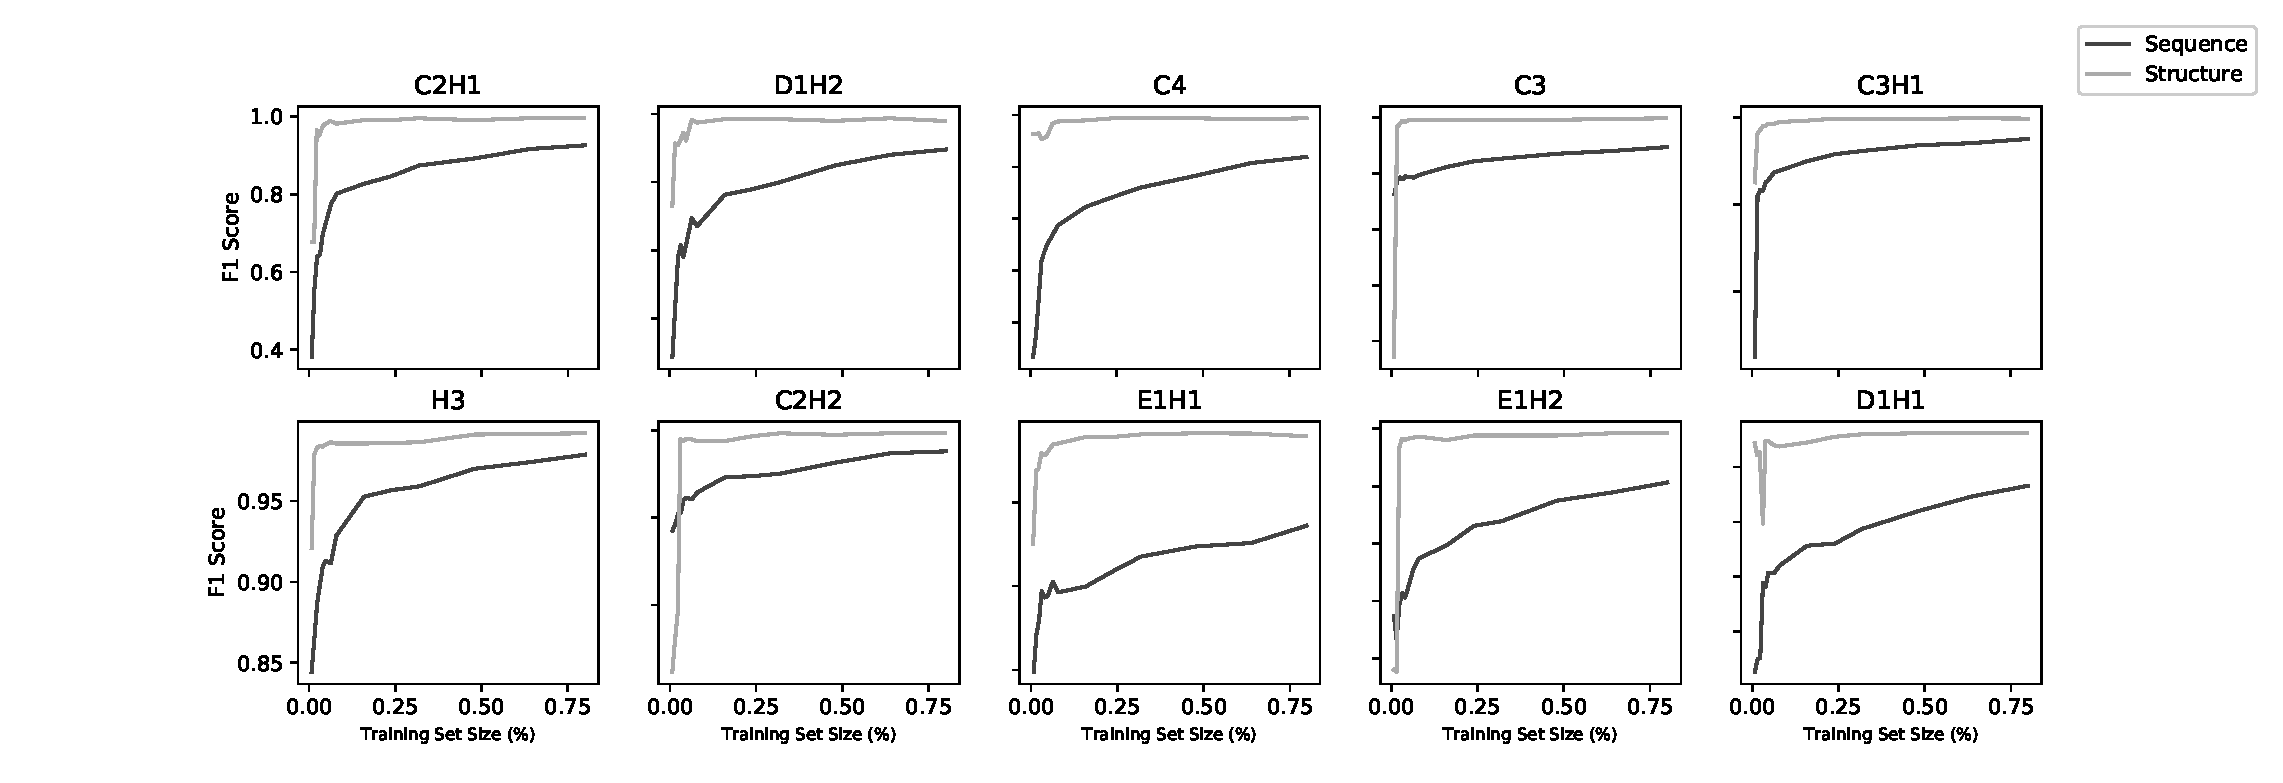
\includegraphics[width=1.0\textwidth]{Figures/learning-curve.eps}
\caption{\label{fig:learning-curves} Learning curves for all 20
  models. Each model was trained on increasing subsets of the overall
  training set using five-fold cross-validation. Sequence models
  improved with increasing dataset size, suggesting smaller dataset
  sizes would not be feasible, whereas structure models did not.}
\end{figure}

While the training is affected by dataset size, this does not appear to be a significant limiting factor for most of the models here. Figure~\ref{fig:size-score} shows the model performance (as MCC) for the sequence and structure models. The performance of the sequence models falls off as the dataset falls below a threshold number of data points in the low thousands --- as does the performance of the structural models. The lowest three performing structural models were also the lowest three in dataset size (C3, E1H1, D1H1), but two of these have only two residues so, as discussed above, the performance might not be expected to be very good.

Learning curves (Figure~\ref{fig:learning-curves}) using fractions of the datasets show a correlation with dataset size for the sequence models, but above around 1000 sequences, the structure models do not improve with larger datasets.

The level of abstraction used to describe both sequences and structures made it unlikely that any homology between data in the training and testing sets would artificially improve the performance. The features are largely calculated from residues around the binding residues, rather than the sequence in which they occur. However given the presence of similar sequences in the dataset, I thought it prudent to confirm that these were not artificially increasing the models' performance.

To this end, I wanted to explore what would happen if only unique sequences were used, whereby the available sequences are clustered on some similarity threshold, and one representative from each used. Different sequence identity thresholds were used for clustering with CD-HIT and a training set was created from this new set of sequences for each threshold, and used to create a model. When clustering at 40\% sequence identity (the lowest used), there was slightly lower performance but clustering at this level did result in smaller datasets. As indicated previously, this is a major determinant of these sequence models' performance, so I wanted to determine if this lowered performance was because the dataset size was smaller (which would mean the original models trained on all the data were not compromised) or if a model trained on unique sequences performed less well, which would call into question the high scores of my models as being due to such sequences.

\begin{figure}
\centering
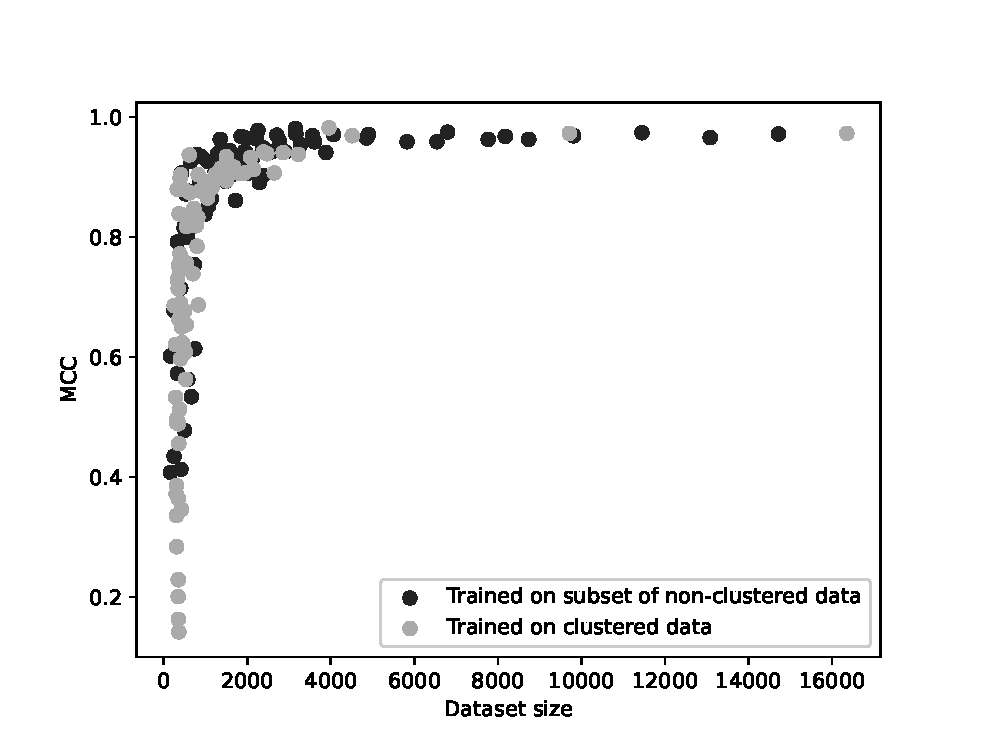
\includegraphics[width=1.0\textwidth]{Figures/clustering.eps}
\caption{\label{fig:clustering} MCC as a function of dataset size for
  160 different models.
  For each of the ten zinc-binding families, we trained a
  classifier on 20\%, 30\%, 40\%, 50\%, 60\%, 70\%, 80\%, 90\% and
  100\% of the original, unclustered data, and also a classifier
  trained on data with sequences clustered by 40\%, 50\%, 60\%, 70\%,
  80\%, 90\% and no clustering. Each of these models is shown here,
  with their performance (MCC) and size of the dataset used to train
  them. The two modes of dataset reduction are shown by different
  shades and it can be seen that the curves are not significantly
  different. A
  model's performance is a function of its dataset size, regardless of
  whether any removal of similar sequences is performed.}
\end{figure}

In order to identify whether this lowered performance was because the models performed worse without the possibility of homologous sequences between the training and test sets, or whether it was a result of the smaller training set,
for each zinc-binding family I trained a classifier on 20\%, 30\%, 40\%, 50\%, 60\%, 70\%, 80\%, 90\% and 100\% of the
original, unclustered data, and also a classifier trained on data with sequences clustered by 40\%, 50\%, 60\%, 70\%, 80\%, 90\% and with no clustering. The performance of the models was then plotted against the resulting dataset sizes as shown in Figure~\ref{fig:clustering}.  This demonstrates that it is dataset size that determines model performance, regardless of the similarity of the sequences in the training and testing datasets. For a given dataset, you could predict how well the model trained on it would perform based on dataset size alone --- the similarity of the sequences within that dataset made no difference when dataset size was held constant.

\begin{table}
  \caption{\label{tab:psiblast}Predictive ability of using BLAST alone
    to predict zinc binding in protein sequences using homology
    alone.}
\begin{center}
\begin{tabular}{llllll} \hline
Family & Dataset Size & Recall & Precision & F1    &  MCC  \\ \hline
C2H2   & 3960         & 0.99   & 0.95      & 0.97  &  0.94 \\
C3H1   & 9710         & 0.29   & 0.87      & 0.44  &  0.33 \\
C2H1   & 2154         & 0.24   & 0.88      & 0.37  &  0.3  \\
D1H1   & 818          & 0.05   & 0.8       & 0.09  &  0.11 \\
C3     & 2868         & 0.13   & 0.61      & 0.21  &  0.07 \\ 
E1H1   & 828          & 0.06   & 0.62      & 0.11  &  0.06 \\
D1H2   & 2470         & 0.03   & 0.53      & 0.06  &  0.01 \\
H3     & 5058         & 0.01   & 0.19      & 0.02  & -0.1  \\
E1H2   & 2648         & 0.02   & 0.33      & 0.04  & -0.06 \\ \hline
\end{tabular}
\end{center}
\end{table}

As an additional means of showing how little effect sequence similarity has on ability to predict zinc binding, I compared the sequence models with using BLAST for predicting zinc-binding sites. For each zinc-binding family, a BLAST database was created using 80\% of the available zinc-binding sequences, and BLAST's ability
to identify zinc binding sites from the remaining 20\% was compared against an equivalently sized negative set. Results are shown in Table~\ref{tab:psiblast}. With the exception of C2H2, using BLAST to find zinc binding based on homology performs much worse than the models presented here. Even in the case of C2H2, which seems to have much more similar sequences in its dataset, my model still narrowly outperforms BLAST.

However the models presented here are not intended to be general purpose zinc binding predictors that detect common properties of all zinc binding sites --- they are family-specific predictors based on the principle that common, specific types of zinc binding site have more identifiable, consistent properties than do zinc binding sites in general. As a result, they will not readily detect binding sites of uncommon zinc-binding families. This abstract predictiveness has been deliberately discarded to create highly effective models for specific, common families of zinc binding sites. It is also noteworthy that the binding site itself is a useful unit of prediction using this
methodology --- even for sequences --- rather than individual binding sites. The models are therefore identifying something biologically real (a zinc binding site) rather than something which does not actually exist in isolation (a single zinc binding residue), but which is a useful heuristic in some circumstances.

\begin{table}
  \caption{\label{tab:genome}Percentage of genome predicted to be zinc
    binding by ZincBindPredict for an assortment of bacterial
    genomes. Genomes were acquired from ensembl
    \cite{yates2020ensembl} in the form of translated polypeptide
    sequences, with a sequence labelled as zinc binding if any of the
    ten models finds at least one zinc binding site for that
    sequence/family combination. See Supplementary file {\tt
      genomes.zip} for the full results.}
\begin{center}
\begin{tabular}{ll} \hline
Species                          & Percentage of Genome   \\
                                 & Predicted Zinc Binding \\ \hline
{\it Campylobacter jejuni}       & 6.4\%                  \\
{\it Clostridioides difficile}   & 5.8\%                  \\
{\it Enterococcus faecalis}      & 7.5\%                  \\
{\it Listeria monocytogenes}     & 7.9\%                  \\
{\it Mycobacterium tuberculosis} & 11.3\%                 \\
{\it Salmonella enterica}        & 11.1\%                 \\
{\it Shigella flexneri}          & 10.1\%                 \\ 
{\it Streptococcus pneumoniae}   & 7.6\%                  \\ \hline

\end{tabular}
\end{center}
\end{table}

A demonstration of this can be seen by applying the sequence models to bacterial genomes to measure the proportion of typical genomes that the models predict to be zinc binding, as shown for a range of bacterial genomes in Table~\ref{tab:genome}. For most genomes, fewer than 10\% of proteins are flagged as zinc binding, with the average for the genomes examined being 8.46\%. Given that the zinc-binding families for which predictors have been generated represent 67.0\% of binding sites in ZincBindDB, this would imply a `true' predicted proportion of 12.6\% which is a little higher than the widely cited figure of 10\%.

\section{Access to Models}

The models are available through a web app called ZincBindPredict. This is a GraphQL API, like the ZincBindDB database API, which allows users to submit jobs and get the results. A GraphQL request can be sent with either a protein sequence or protein structure, and a job ID will be returned (see Figure~\ref{fig:zbp-mutation}). This can then be polled for results as the protein or sequence is searched using each model in turn, with the identified binding sites returned as a list with the associated probability (see Figure~\ref{fig:zbp-query}). Internally, when a protein is submitted a `job' folder is created, using the current UNIX time in milliseconds as the ID. This job ID is returned to the user, which they can use to query the status of the job, as a script which runs each of the model in turn runs as a background process and saves its results to the job's folder on the server, for inspection by the API.

The ZincBind web interface that was explored in-depth in Chapter 3 also has a page that allows users to submit jobs using a more human-friendly interface, which itself consumes the ZincBindPredict API (see Figure~\ref{fig:prediction-interface}). The user is prompted to provide the representation of a protein - either as a structure file, a sequence file, or a FASTA sequence pasted in. They also have the option of only searching for specific families. Positive results are listed on a results page once the job is complete, and the number of rejected residue combinations is listed.

\begin{figure}
\centering
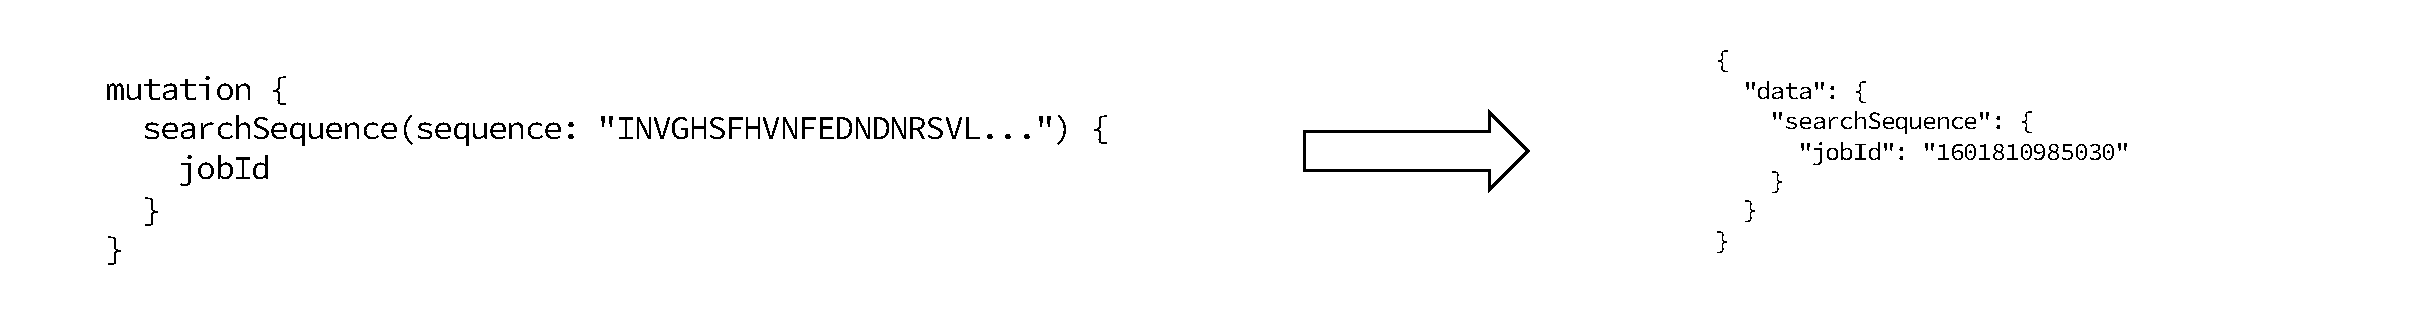
\includegraphics[width=1.0\textwidth]{Figures/zbp-mutation.eps}
\caption{\label{fig:zbp-mutation} A mutation from the ZincBindPredict API. Mutations
begin with the mutation identifier to indicate that the top level \texttt{Mutation} object
is what the \texttt{searchSequence} mutation belongs to --- queries can begin with
\texttt{query} too but this is optional. Here the sequence is being given as an
argument, and the ID of the job is returned.}
\end{figure}

\begin{figure}
\centering
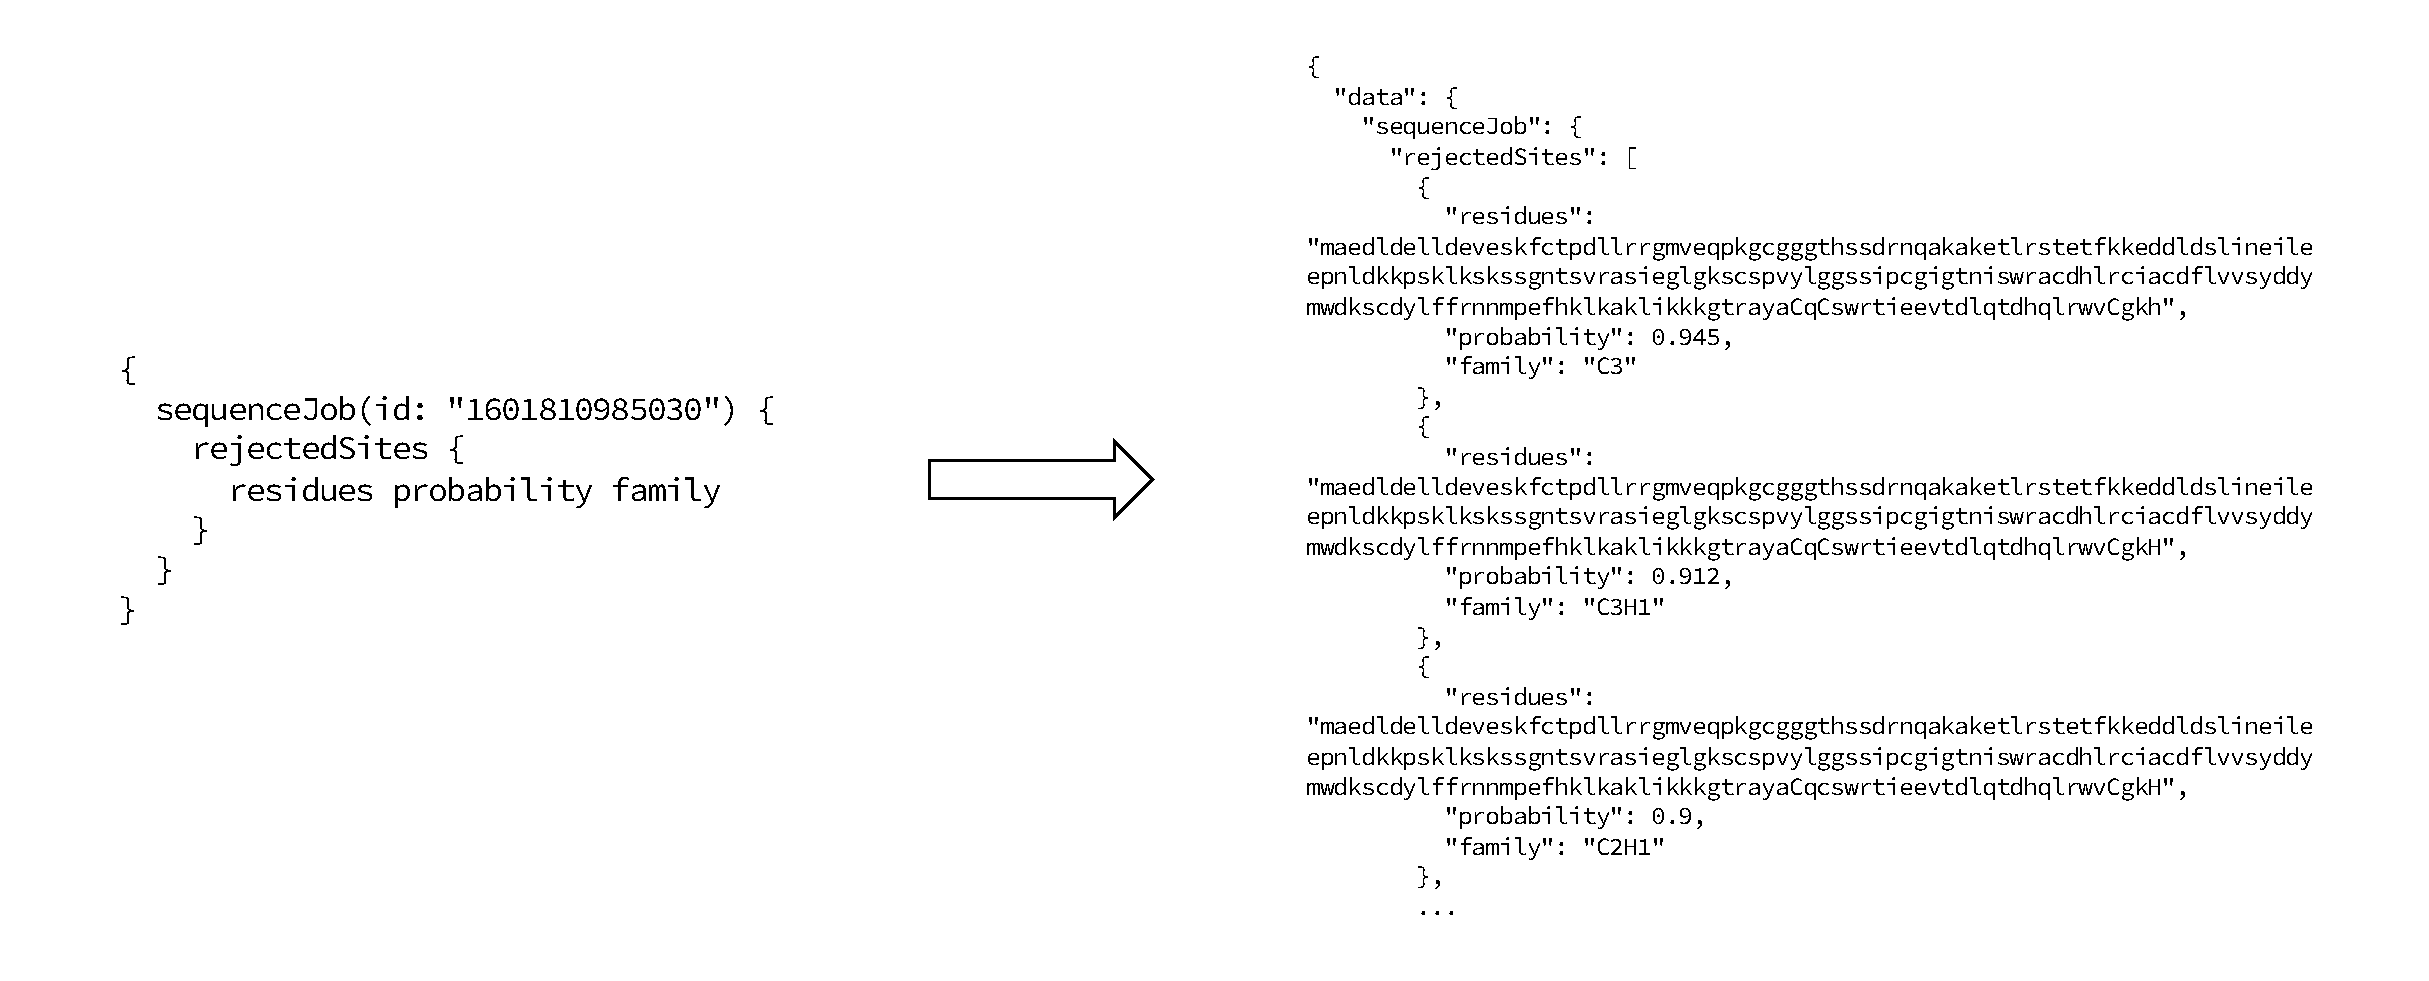
\includegraphics[width=1.0\textwidth]{Figures/zbp-query.eps}
\caption{\label{fig:zbp-query} A query for the results of a ZincBindPredict job.
The ID of the job is supplied, and this particular query requests the status of
the job, as well the predicted sites. The rejected sites can also be requested,
but since they are quite numerous, typically the flexibility of GraphQL in allowing
you to choose to omit them is useful in conserving network resources.}
\end{figure}

\begin{figure}
\centering
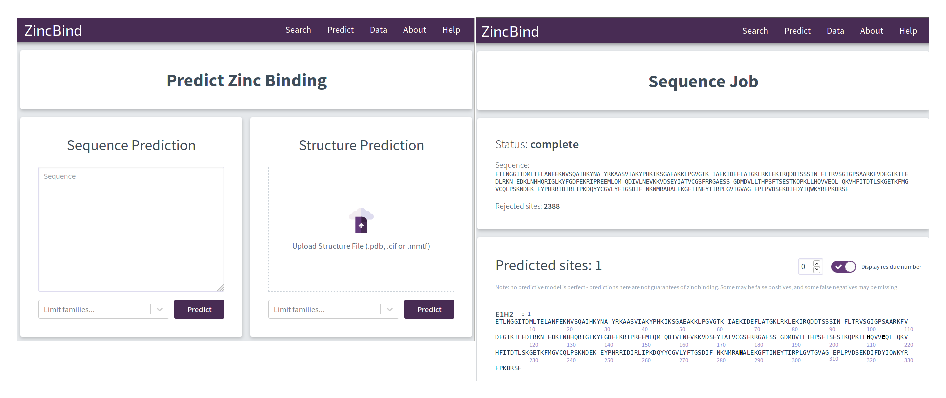
\includegraphics[width=1.0\textwidth]{Figures/prediction-interface.eps}
\caption{\label{fig:prediction-interface} The prediction page on the ZincBind web interface, and an example of a predicted zinc binding site in a protein sequence.}
\end{figure}

\section{Conclusion}

The models created here are highly effective, albeit at a very particular task. They are not predictors of zinc binding in general, and they will not generally detect zinc binding sites of obscure families and residue combinations. They were never intended to. A deliberate trade-off between model effectiveness and model generalisability has been made in order to demonstrate the principal that properties of binding sites within families \emph{are} more tightly distributed and hence create more accurate models. These models also detect something biologically real --- full binding sites --- rather than individual zinc binding residues which, as discussed, are an artificial concept.

However, this downside is not necessarily permanent. The models are limited to these ten models because these are the families for which there is sufficient (only just, in the case of some of the sequence models) data to train a classifier. However, the data in ZincBind is constantly growing thanks to the automated database update scripts in place. Over the time, the eleventh-placed model will acquire enough data to warrant a model, and then the twelfth, and so on. The dataset-size threshold for training is not relative to the total size of the database, it is an absolute amount, and so over time more and more families will be able to have models trained for them, and the models will become more comprehensive of zinc binding generally. The benefits of this trade-off are permanent --- the deficiencies are temporary.






